
Auf der Profilseite werden ein Profilbild, ein Hintergrundbild und für das Matching relevante persönliche Informationen dargestellt. Es gibt eine Version, die nur von anderen Nutzern sichtbar ist, mit denen ein Match stattgefunden hat, und eine Version, die über die Bottom-Navigation-Bar erreichbar werden kann. Die Letztere wird in Abbildung \ref{fig:profilseite_alle} dargestellt und unterscheidet sich von der Version für andere Nutzer darin, dass Profil- und Hintergrundbild bearbeitet werden können.\\
Das Farbschema und das Design wurden an die bisherigen Seiten angepasst. Um die Oberfläche simpel und selbsterklärend zu halten, wird jede dargestellte Information mit einem passenden Icon und einem Hinweis versehen (siehe Abbildung \ref{fig:profilseite_a}). Die Icons zum Bearbeiten der Bilder sind, wie auch in vielen anderen Apps, platziert und designt. Sie öffnen die systemeigene Bildergalerie des Smartphones um den Nutzer aus einem bekannten Umfeld Bilder auswählen lassen zu können.\\
Beim initialen Öffnen einer Profilseite sollen Namen, Profilbild und ein Hintergrundbild ins Auge springen. Sie stellen die ersten Informationen dar, die dem Betrachter wichtig sind, weshalb sie wie in Abbildung \ref{fig:profilseite_a} deutlich sichtbar ist  beim Öffnen mehr als die Hälfte des Bildschirms einnehmen. Anschließend wird der Fokus auf detailliertere Informationen gerichtet. Auf der Profilseite von StreamSwipe wird hierfür heruntergescrollt um den Block mit den Profildaten sehen zu können. Bei dieser Aktion blendet eine Animation das Profilbild aus und verschmälert das Hintergrundbild. Der Benutzername wird ebenfalls aus dem Fokus gezogen, bleibt aber wie in Abbildung \ref{fig:profilseite_b} zu sehen mit dem verbleibenden Hintergrundbildausschnitt erhalten. Dies hilft dem Betrachter unterbewusst bei dem Fokuswechsel und schafft ein modernes, responsives Feedback bei der User Experience.\\
Um das durchgängig schlichte Design der App zu erhalten ist der Zugang zu den Einstellungen ausschließlich auf der Profilseite zu finden. Hierfür ist im rechten oberen Bildschirmbereich das repräsentative Icon. Der hierdurch erreichbare Bildschirm (Abbildung \ref{fig:profilseite_c}) ist gleich aufgebaut wie die Informationeneingabe nachdem ein neuer Account erstellt wurde (Abbildungen \ref{fig:login_c} und \ref{fig:login_d}). Die dort angegebenen Informationen können hier wieder angepasst werden. %TODO Referenz auf account erstellen bild


\begin{figure}[tbt]
	\begin{subfigure}{0.33\textwidth}
	\centering
	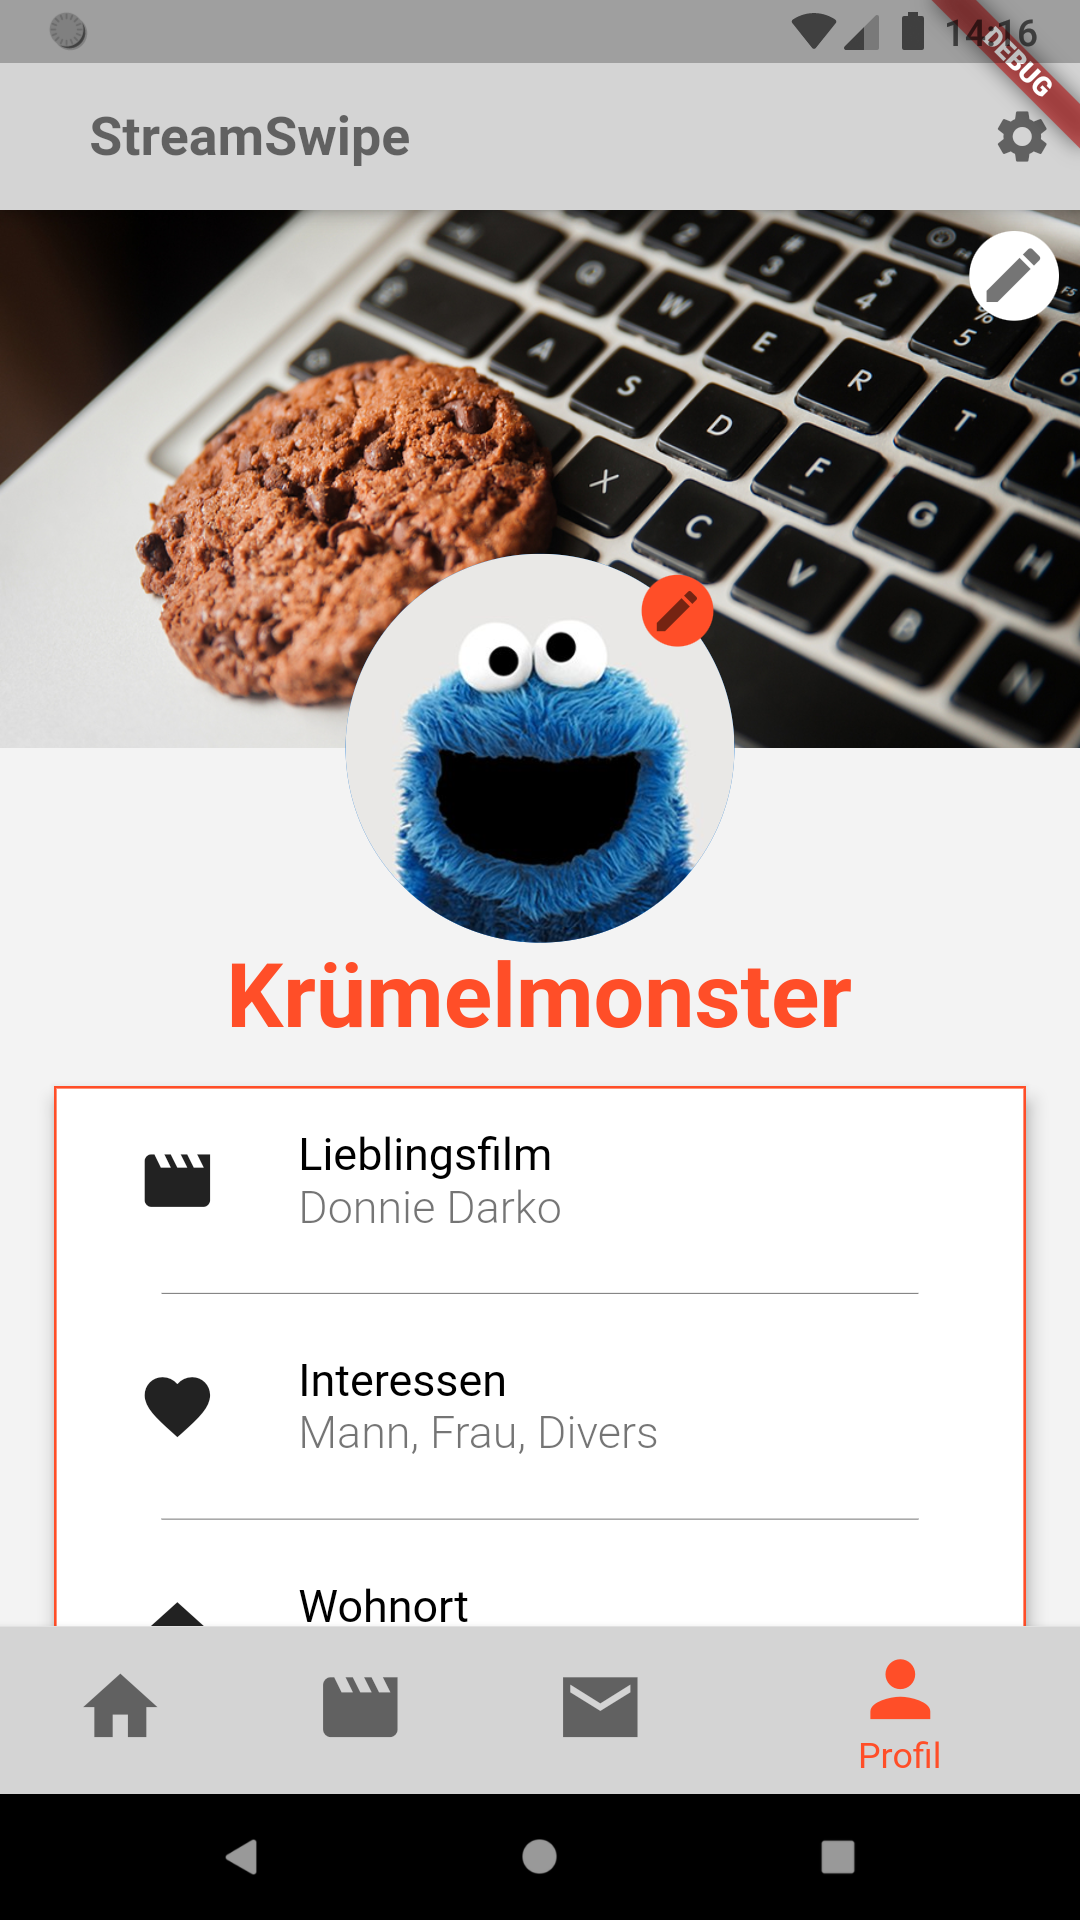
\includegraphics[scale=0.13]{Benutzeroberfläche/images/screenshot_profilseite_1.png}
	\caption{}
	\label{fig:profilseite_a}
	\end{subfigure}
	\begin{subfigure}{0.33\textwidth}
	\centering
	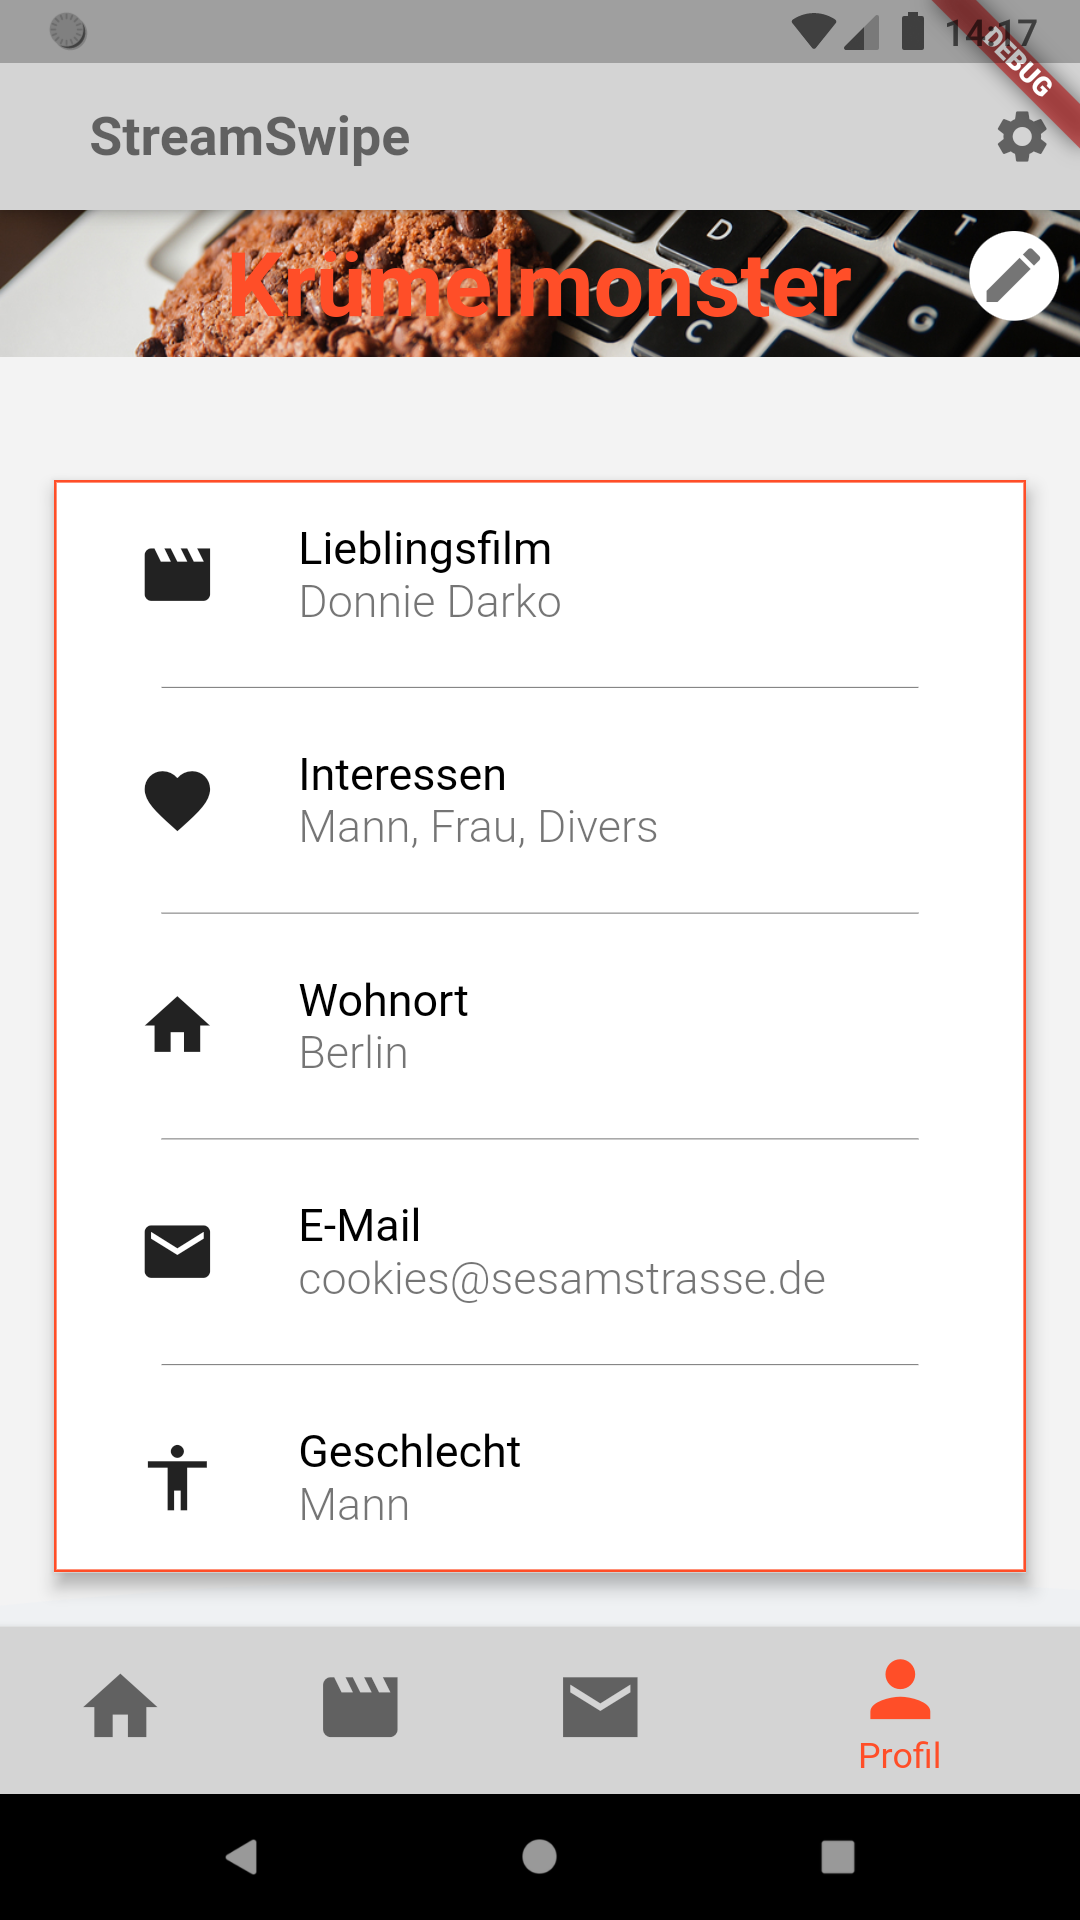
\includegraphics[scale=0.13]{Benutzeroberfläche/images/screenshot_profilseite_2.png}
	\caption{}
	\label{fig:profilseite_b}
	\end{subfigure}
	\begin{subfigure}{0.33\textwidth}
	\centering
	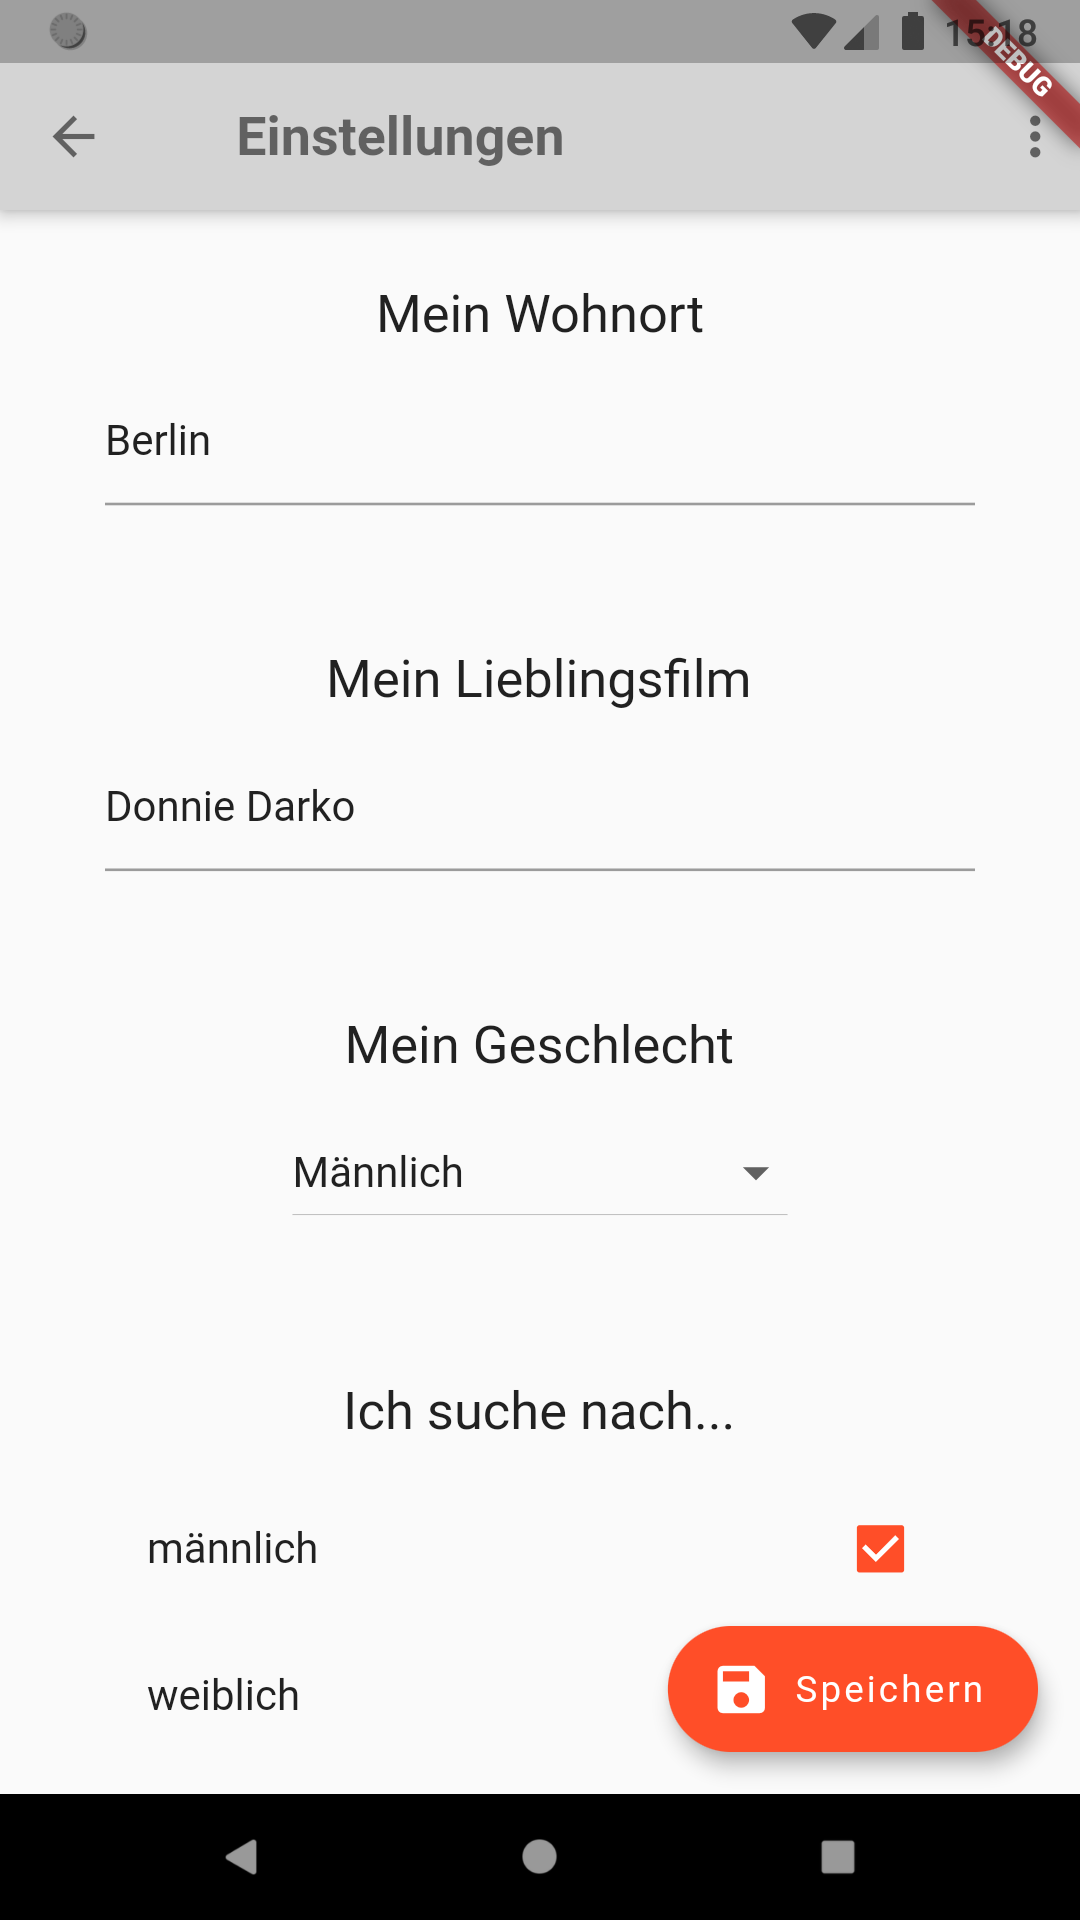
\includegraphics[scale=0.13]{Benutzeroberfläche/images/screenshot_profilseite_3}
	\caption{}
	\label{fig:profilseite_c}
	\end{subfigure}
\caption[Screenshots der Profilseite]{Profilseite wie sie für den Nutzer selbst angezeigt wird (a) im normalen Zustand und (b) nach vollständigem Einklappen des Profilkopfes durch eine Animation während dem Herunterscrollen. Mit den von hier aus erreichbaren Einstellungen (c) können die anfänglich gegebenen Profilangaben abgepasst werden.}
\label{fig:profilseite_alle}
\end{figure}
